\documentclass{article}
\usepackage{tikz}
\usetikzlibrary{scopes}

\begin{document}


%\tikzstyle{block} = [draw, rectangle, minimum width = 2, minimum height = 2]

\hspace*{-8em}
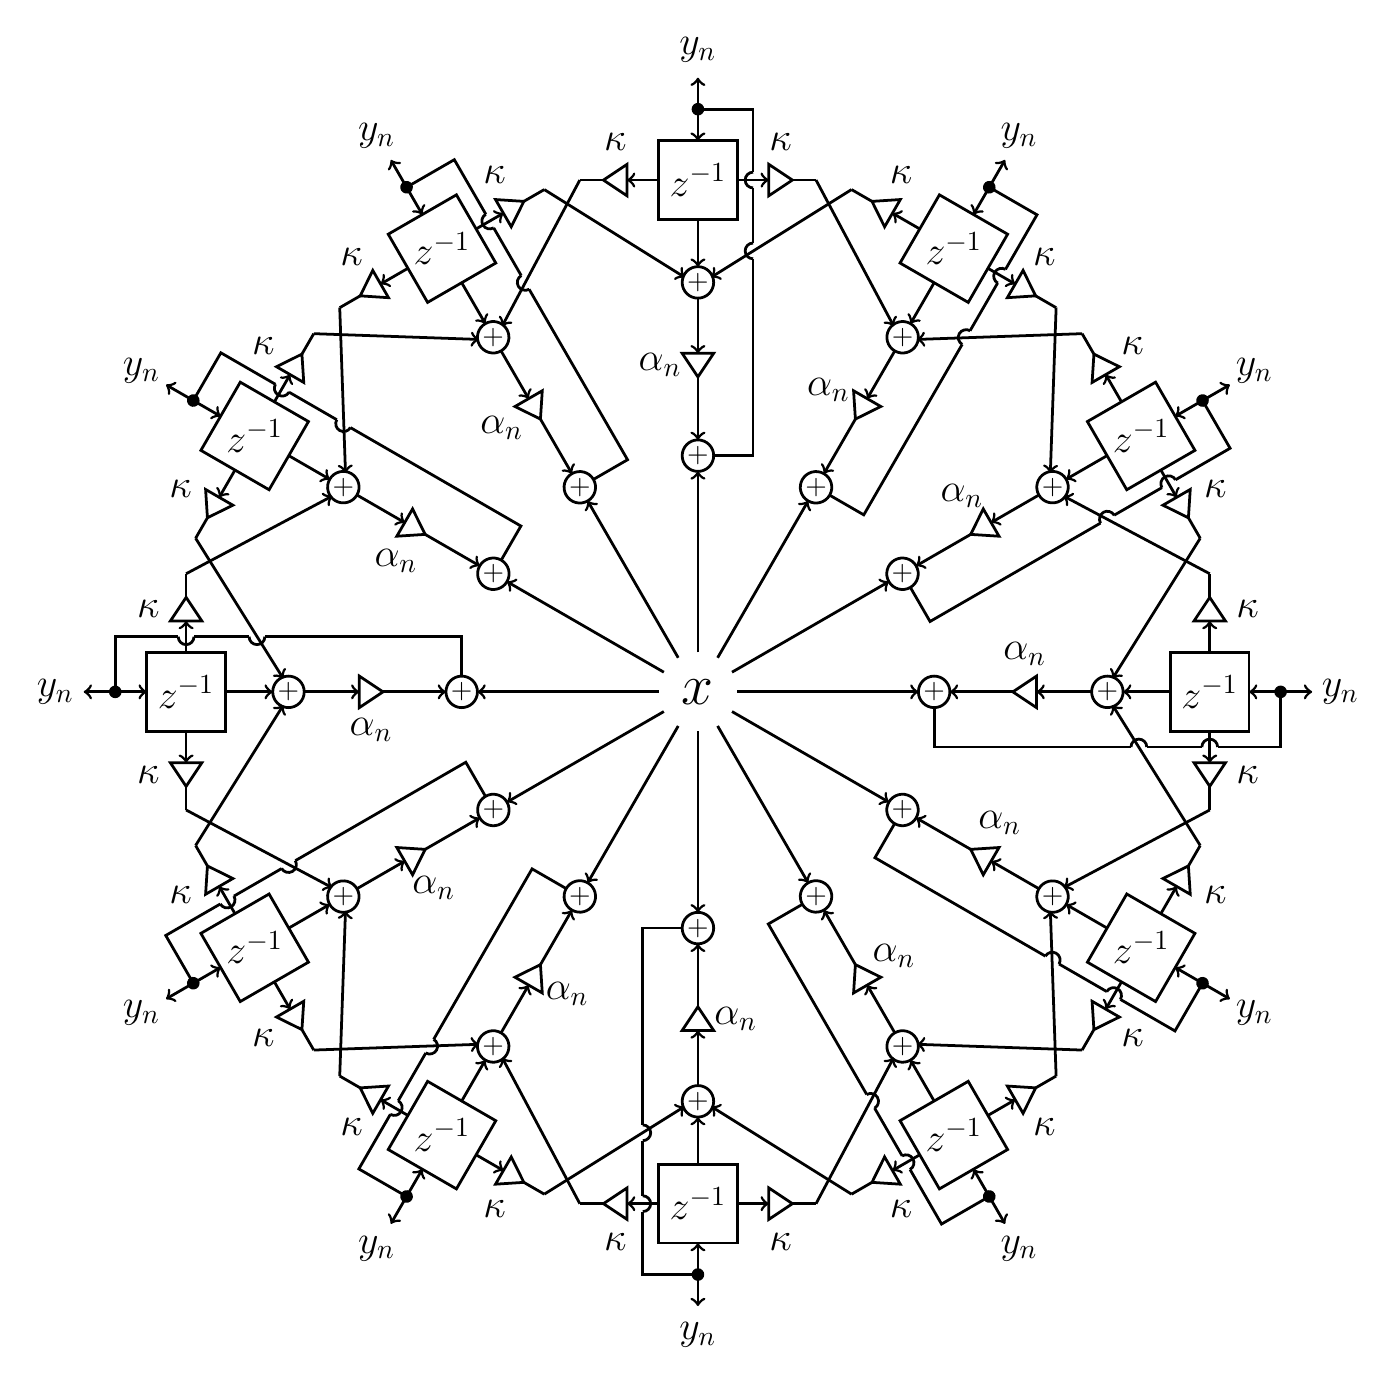
\begin{tikzpicture}[line width=1pt]

    \def\unit_delay{
      \filldraw[fill=white,draw=black, line width=1pt,sharp corners] (-0.5,-0.5) -- (-0.5,0.5) -- (0.5,0.5)  -- (0.5,-0.5) -- cycle;
      \draw(0,0) node {\Large$z^{-1}$};
    }

    \def\factor#1{
      \filldraw[fill=white,draw=black, line width=1pt,sharp corners] (-0.15,-0.2) -- (-0.15,0.2) -- (0.15,0) -- cycle;
      \draw(0.,.48) node {\Large #1};
    }

    \def\factorl#1{
      \filldraw[fill=white,draw=black, line width=1pt,sharp corners] (-0.15,-0.2) -- (-0.15,0.2) -- (0.15,0) -- cycle;
      \draw(0.,-.48) node {\Large #1};
    }

    \def\factorr#1{
      \filldraw[fill=white,draw=black, line width=1pt,sharp corners] (-0.3,-0.45) -- (-0.3,0.45) -- (0.4,0) -- cycle;
      \draw(-0.05,0) node {\large #1};
    }

    \def\xline#1{
      \draw[->] (0,0) -- (#1,0);
    }

    \def\coupling{
      \begin{scope}[ shift = ({ 0.0 ,  0.3 })  , rotate =  90  ] \xline{.6}           \end{scope}
      \begin{scope}[ shift = ({ 0.0 ,  1.05 })  , rotate =  90  ] \factorl{$\kappa$}   \end{scope}
      \draw (0,1.2) -- (0,1.5);
      \begin{scope}[ shift = ({ 0.0 ,  1.50 }) , rotate =  152 ] \xline{2.1}          \end{scope}
      \begin{scope}[ shift = ({ 0.0 , -0.3 })  , rotate = -90  ] \xline{.6}           \end{scope}
      \begin{scope}[ shift = ({ 0.0 , -1.05 })  , rotate = -90  ] \factor{$\kappa$}   \end{scope}
      \draw (0,-1.2) -- (0,-1.5);
      \begin{scope}[ shift = ({ 0.0 , -1.50 }) , rotate = -152 ] \xline{2.1}          \end{scope}
    }

    \def\dot#1{
      \fill(0,0) circle(#1);
    }

    \def\adder{
      \draw circle(0.2);
      \node(0,0) {$+$};
    }

    \def\output{
      \draw     (0,0) -- (0,1);
      \draw[->] (0,1) -- (2,1) node[pos=1.2] {\huge $y_n$};
    }

    \def\feedback{
      \draw     (0,-.2) -- (0,-.7) -- (2.5,-.7);
      \draw     (2.7,-.7) -- (3.4,-.7);
      \draw     (2.7,-.7) arc(0:180:0.1);
      \draw     (3.6,-.7) -- (4.4,-.7) -- (4.4,0);
      \draw     (3.6,-.7) arc(0:180:0.1);
      \draw[->] (4.4,0) -- (4.0,0);
      \draw[->] (4.4,0) -- (4.8,0) node[pos=1.9] {\Large $y_n$};
      \fill(4.4,0) circle(.08);
    }


    \node(0,0) { \huge $x$ };

    %\foreach \phi in{0,24,...,336}
    \foreach \phi in{0,30,...,330}
    \begin{scope}[ rotate = \phi ]
      \begin{scope}[ shift = ({ 0.5 , 0 }) ]                \xline{2.3}           \end{scope}
      \begin{scope}[ shift = ({ 3.0 , 0 }) ]                \adder                \end{scope}
      \begin{scope}[ shift = ({ 3.0 , 0 }) ]                \feedback           \end{scope}
      \begin{scope}[ shift = ({ 4.0 , 0 }) , rotate = 180 ] \xline{0.8}           \end{scope}
      \begin{scope}[ shift = ({ 4.15 , 0 }) , rotate = 180 ] \factorl{$\alpha_n$}   \end{scope}
      \begin{scope}[ shift = ({ 5.0 , 0 }) , rotate = 180 ] \xline{.7}            \end{scope}
      \begin{scope}[ shift = ({ 5.2 , 0 }) ]                \adder                \end{scope}
      \begin{scope}[ shift = ({ 6.0 , 0 }) , rotate = 180 ] \xline{.6}            \end{scope}
      \begin{scope}[ shift = ({ 6.5 , 0 }) ] \coupling           \end{scope}
      \begin{scope}[ shift = ({ 6.5 , 0 }) ]                \unit_delay           \end{scope}
      %\begin{scope}[ shift = ({ 5.2 , 0 }) ] \dot{.1}              \end{scope}
      %\begin{scope}[ shift = ({ 5.2 , 0 }) ] \output            \end{scope}
      %\begin{scope}[ shift = ({ 5.3 , 0 }) ] \xline{.6}            \end{scope}
    \end{scope};


\end{tikzpicture}
\end{document}

